\chapter{Experiments}\label{cha:experiments}

\section{Simulator}\label{sec:simulator}

We created a symulator to generate distorted points. We used it to test the
solver, and test the correctness of projection and back-projection points.

\section{Metrics}\label{sec:metrics}

\begin{itemize}
	\item Reprojection error
	\item Number of detected corners
\end{itemize}

\section{Dataset}\label{sec:dataset}

For the project, we need highly distorted photos of calibration boards. It takes
a lot of work to generate such a dataset, as cameras which produce such images are
usually expensive. Therefore, it would be preferable to use an existing dataset.

\textcite{lochmanBabelCalibUniversalApproach2021} collected a wide number of
datasets, typically used in the field for the benchmarking of the camera
calibration. They're provided in a Deltille \cite{DeltilleDetector2023} format,
and are well documented:

\textbf{Kalibr} contains several established datasets that are commonly used for testing
the accuracy of camera calibration frameworks: Double Sphere
\cite{usenkoDoubleSphereCamera2018}, EuRoC \cite{burriEuRoCMicroAerial2016}, TUM
VI \cite{schubertTUMVIBenchmark2018}, and ENTANIYA 1
\cite{Calibration250degFisheye}.
The Kalibr calibration framework was used in the
original publications cited above, hence the name of the dataset.
As a calibration pattern, AprilGrid with 6x6 tags of 88 mm size was used.
In total, the datasets contain approximately 800 images.

\textbf{OCamCalib} \cite{scaramuzzaFlexibleTechniqueAccurate2006} is a dataset
of approximately 300 images.
As a calibration pattern, the checkerboard pattern of different sizes was used.

\textbf{UZH} \cite{AreWeReady} is a dataset of approximately 800 images
collected using the following cameras:
As a calibration pattern, AprilGrid with 4x5 tags of 75 mm size was used.
The dataset contains approximately 800 images.

\textbf{OV} \cite{duisterhofTartanCalibIterativeWideAngle2022} is a dataset of
approximately 1400 images. It was collected using eight stereo cameras.
As a calibration pattern, the checkerboard pattern with 9x6 tags of 22 mm size
was used.

\textcite{duisterhofTartanCalibIterativeWideAngle2022} also provide their
dataset from the TartanCalib project, but it is quite challenging to use it as it
comes in the Robot Operating System (ROS) .bag format.

\begin{figure}[h!]
	\centering
	\begin{subfigure}[b]{0.3\linewidth}
		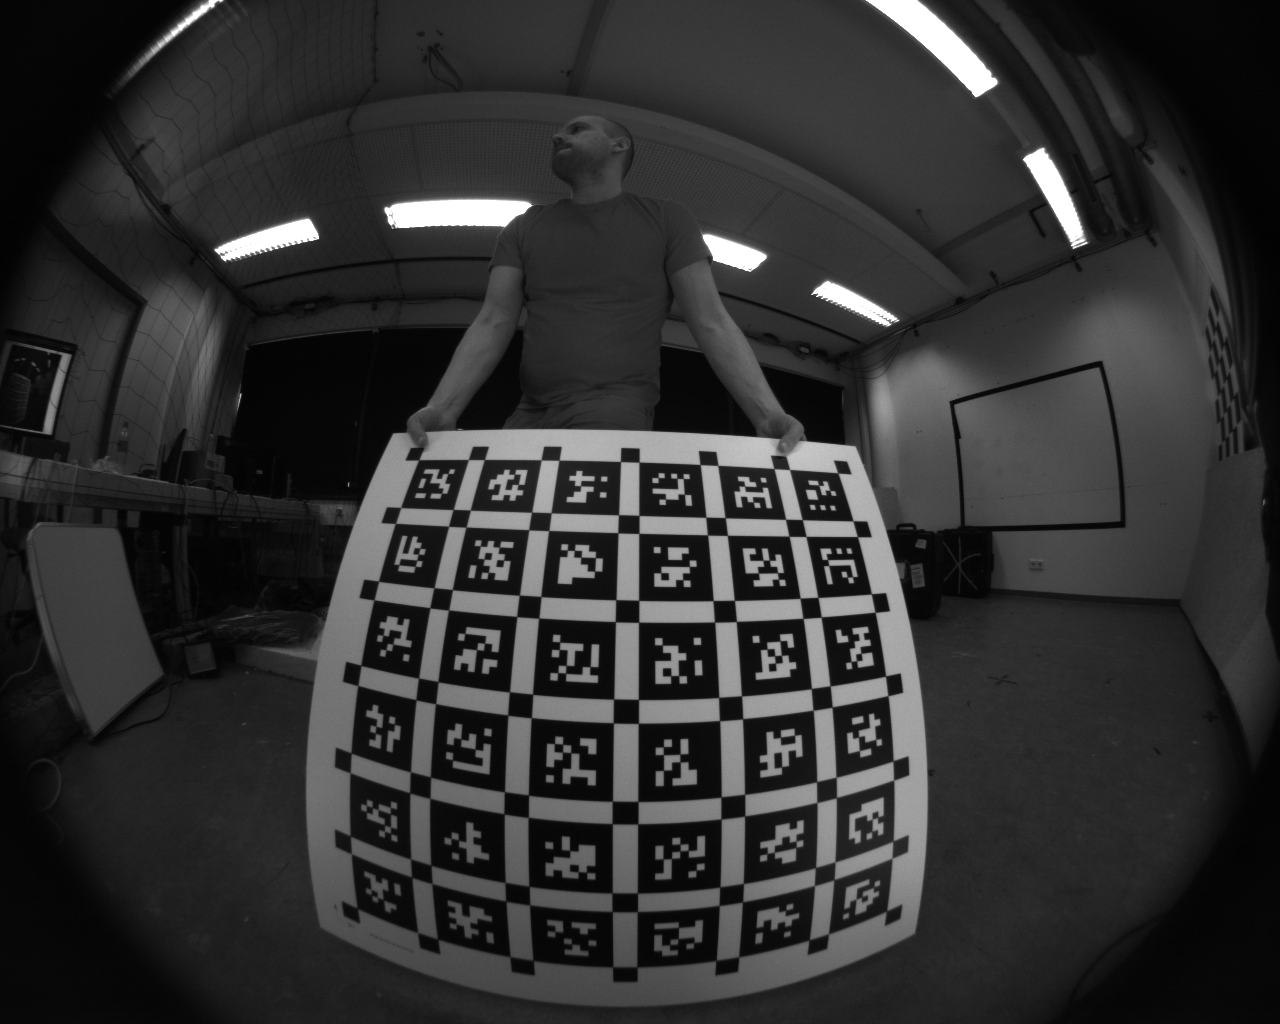
\includegraphics[width=\linewidth]{Kalibr.png}
		\caption{Kalibr}
	\end{subfigure}
	\hfill
	\begin{subfigure}[b]{0.3\linewidth}
		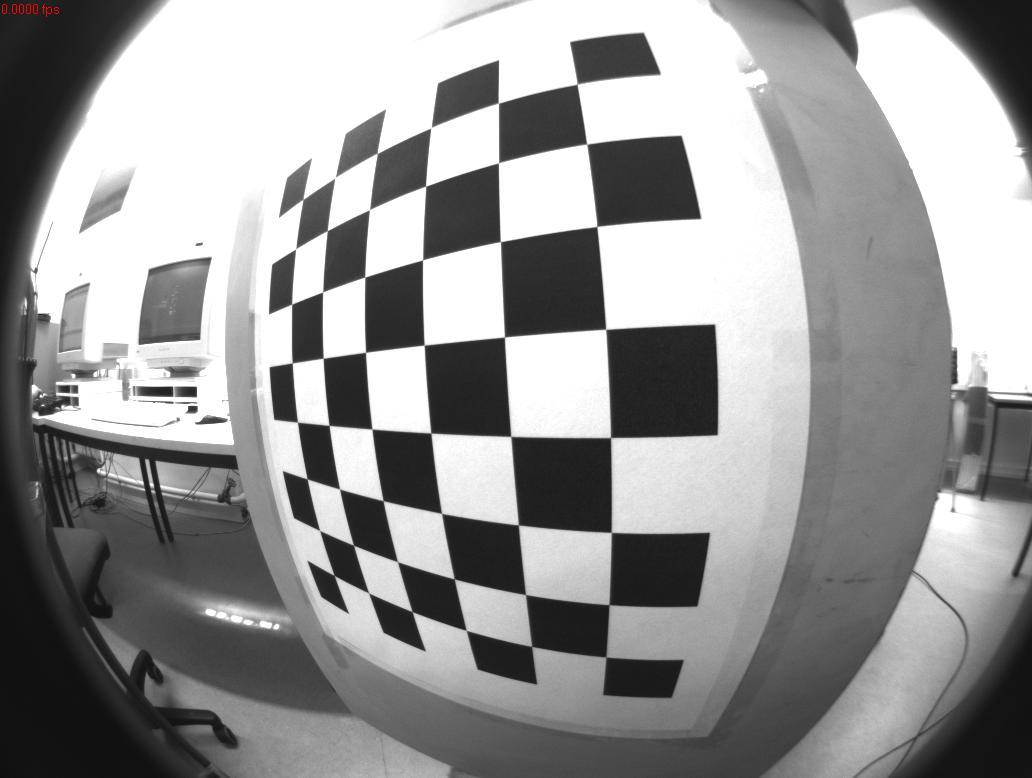
\includegraphics[width=\linewidth]{OCamCalib.png}
		\caption{OCamCalib}
	\end{subfigure}
	\hfill
	\begin{subfigure}[b]{0.3\linewidth}
		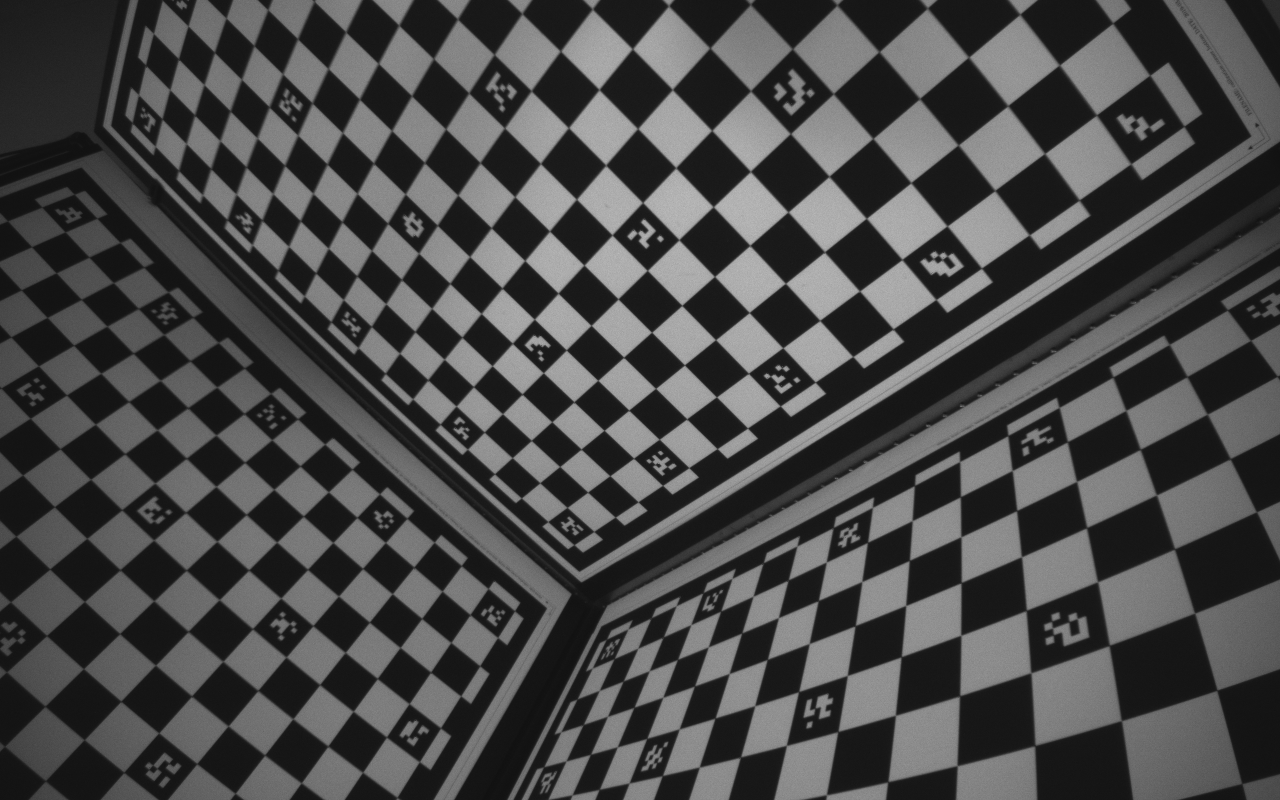
\includegraphics[width=\linewidth]{OV.png}
		\caption{OV}
	\end{subfigure}
	\begin{subfigure}[b]{0.3\linewidth}
		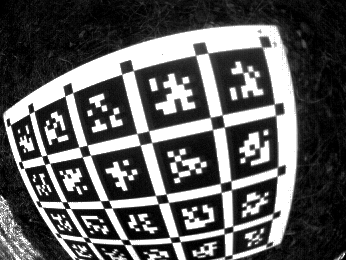
\includegraphics[width=\linewidth]{UZH.png}
		\caption{UZH}
	\end{subfigure}
	\begin{subfigure}[b]{0.3\linewidth}
		\includegraphics[width=\linewidth]{tartancalib.png}
		\caption{TartanCalib}
	\end{subfigure}
	\caption{Images from the datasets}
\end{figure}

\todo{Probably, remove everything but BabelCalib, as we didn't use AprilGrid}


